This chapter describes the final part of this work\textemdash creating a proof-of-concept implementation of the plugin.
Initially, we chose the third implementation option described in \autoref{subsec:encryption-key-derived-from-a-signature}.
However, we later discovered that our initial analysis missed one crucial detail. The section 6.1.1 of \glsxtrshort{webauthn} specification
introduces an optional \emph{signature counter}~\cite{fido:webautn}:

\begin{quoting}
	Authenticators SHOULD implement a signature counter feature. The signature counter is incremented
	for each successful authenticatorGetAssertion operation by some positive value, and its value is returned
	to the WebAuthn Relying Party within the authenticator data. The signature counter's purpose is to aid Relying Parties
	in detecting cloned authenticators [\ldots]
\end{quoting}

If an authenticator implements the signature counter, the counter's value is included in metadata that are added
to the \gls{rp}'s challenge before signing it. Supporting this feature is optional, but if an authenticator does support it,
there is no way to prevent its use~\cite{fido:webautn}. That means the resulting signature is different every time, which
breaks one of the essential requirements of our implementation strategy. After this discovery, we were, therefore,
only left with the last option described in \autoref{subsec:key-stored-as-resident-key-metadata}.

\section{Communicating with the authenticator}\label{sec:communicating-with-the-authenticator}

Rather than communicating with the authenticator directly via \glsxtrshort{ctap},
we initially chose to use libfido2 package by Yubico. It handles communication with
a FIDO device over USB and exposes all its features as both a C library
and a command-line tool~\cite{libfido2}.

This choice turned out to be a problem later, as starting with a Windows 10, version 1903,
Microsoft has restricted the direct access to FIDO devices to privileged applications. Applications not running
with administrator privileges have to use a new native \glsxtrshort{api}~\cite{libfido2}.

Requiring administrator privileges to use our plugin would limit its usability and might raise security concerns,
so we attempted to switch to the native API. This has, however, brought several new problems.

First, the only available piece of documentation for this API is a C header file in one of Microsoft's GitHub repositories~\cite{microsoft:webauthn}.
Further, the README file in this repository points back to the \glsxtrshort{webauthn} and \glsxtrshort{ctap} specifications "for more details",
but the exposed interfaces from the header file do not directly match those described in the specifications.

Eventually, we have found that the API does not expose the full functionality to applications that use it.
For example, when an authenticator returns multiple credentials, Windows uses its own graphical interface
to let the user choose which credential they want to use. In this interface, it displays the credential
metadata (\mintinline{csharp}{name} and \mintinline{csharp}{display name}). It does not, however,
expose any metadata to the application.

Because our implementation requires access to the \mintinline{csharp}{icon} field, it cannot
use the native Windows \glsxtrshort{api}, and we have to accept it will only work when running under a privileged account.

At this point, it is fair to say that FIDO2\textemdash at least in its current state\textemdash
did not turn out to be a good choice for the purpose of implementing an alternative database unlocking strategy. Out of the four examined implementation approaches,
we have found that three will not work at all (for the first two, the reasons are explained directly in the initial analysis, for the third one, at the beginning of this chapter),
and the fourth approach\textemdash which was also not ideal from the beginning\textemdash will require administrator privileges to use our plugin,
which might make it impossible to use for some people, create security issues, and overall make the plugin harder to use. In the next section,
we describe a way to partially limit the negative aspects of this requirement, but it is not possible to do so entirely.

\section{Plugin architecture}\label{sec:plugin-architecture}

In this section, we describe the architecture of the plugin, implementing the approach proposed in \autoref{subsec:key-stored-as-resident-key-metadata}.
The chosen architecture consists of two modules:

\begin{itemize}
	\item the KeePass plugin itself, written in C\# and implementing the required interface,
	\item a "device communicator" module, in the form of a native executable file written in C++, which performs the operations that require privileged access.
\end{itemize}

This choice was made for two main reasons. First, because KeePass plugins run in the context of the main KeePass process,
performing the privileged operations directly in the plugin would mean the whole KeePass application
\textemdash and in turn, any other loaded KeePass plugin\textemdash would have to be running with
administrator privileges, breaking the principle of least privilege\footnote{
	This principle says that every program should operate using the least set of privileges it needs to function,
	which limits the damage that can result from an accident or programmer error~\cite{the-protection-of-information}.
}.

Second, because libfido2 is an unmanaged DLL written in C, we would need to create a wrapper class acting as an
intermediary between the unmanaged \glsxtrshort{dll}, and the managed C\# code~\cite{microsoft:unmanaged-dll}.

By implementing the device communicator as a separate executable, we allow the plugin\textemdash and consequently,
KeePass\textemdash to run under a regular account and greatly reduce the amount of code running in a privileged context.

The plugin module extends the KeePass user interface by adding a new entry "KeePassFIDO2 Options" to the "Tools" menu. After selecting this entry,
the user can associate a new authenticator with the currently open database. To do so, they need to click the corresponding button
and perform the regular user verification, as requested by the authenticator. The options window is shown in \autoref{fig:the-plugin-options-window}.

\begin{figure}[H]
	\centering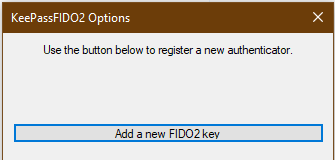
\includegraphics[width=.75\textwidth]{images/plugin-options}
	\caption{The plugin options window}
	\label{fig:the-plugin-options-window}
\end{figure}

Any number of authenticators can be associated with a single database, but for now, it is not possible
to use the same authenticator with multiple databases. This is a limitation that could be removed in future
plugin versions by generating a unique database file identifier, storing it in the database header section
and on the authenticator, and using it to pair a specific database file with the correct credential.

After adding the key, the database can be unlocked by selecting "FIDO2 Key Provider" in the KeePass
unlock dialogue, as shown in \autoref{fig:the-database-unlock-dialogue}.

\begin{figure}[H]
	\centering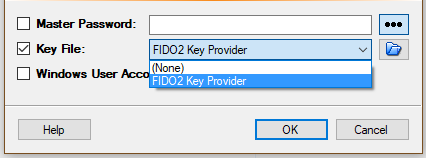
\includegraphics[width=.8\textwidth]{images/plugin-unlock}
	\caption{The database unlock dialogue}
	\label{fig:the-database-unlock-dialogue}
\end{figure}

The communicator module implements two operations. The first is \mintinline{text}{create} to create a new credential,
and the second is \mintinline{text}{get} to retrieve a key stored in an existing credential. These operations are exposed
over a minimal interface that allows passing of the necessary data between the two modules.
\autoref{fig:sequence-diagram-of-a-get-operation} shows how retrieving a stored key looks in this architecture.

\begin{figure}[H]
	\centering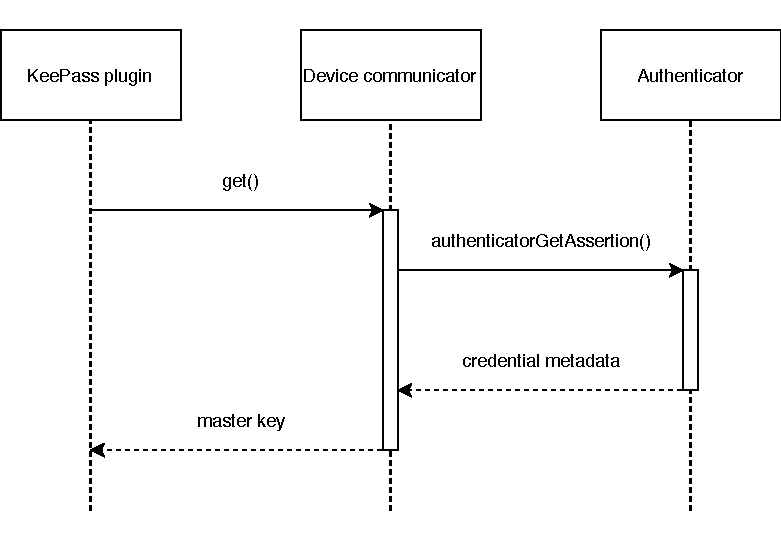
\includegraphics[width=\textwidth]{images/plugin-get}
	\caption{Sequence diagram of a get() operation}
	\label{fig:sequence-diagram-of-a-get-operation}
\end{figure}

Because the exchanged data include the authenticator PIN and the database encryption key,
the primary criteria for choosing the communication channel were security and ease of implementation.

The plugin allocates a buffer where it prepares the PIN and then passes a pointer to this buffer
along with the requested operation name to the communicator via command line arguments. The communicator
reads the prepared buffer, verifies it has the required structure, and in case of the \mintinline{text}{get}
operation, later uses it to pass the retrieved key back to the plugin.

Note that the buffer is allocated within the private memory space of the plugin. This approach takes advantage
of the fact that the communicator is already running as a privileged process and can access the
memory of other processes. Other running unprivileged processes are not able to access this memory.

In the end, this implementation fulfills our initial goal of creating an alternative database unlock strategy
using a FIDO2 device, as well as the design goals described in \autoref{sec:design-goals}. Users can
associate any number of authenticators with their KeePass database, and interchangeably use any of them
or the original unlock method. Associating an authenticator with a database file does not modify it in any way
so that it can still be used with other clients implementing the KDBX file format.

During our work, we used Security Keys by Yubico. The plugin should work
with any other USB authenticator implementing the specifications but was tested only with
the Yubico keys.

An unstated goal of this work was open-sourcing the final implementation and making it freely
available for all KeePass users. Given the previously described issues, however, it should be considered
a proof-of-concept only and may not be suitable for widespread use.
